\section{Theory}

%Explain trilateration
\subsection{Trilateration}
Trilateration makes use of equation \ref{eq_drt} to calculate the distances between the transceivers. 
\begin{equation} \label{eq_drt}
Distance = Rate \times Time
\end{equation}
Since radio signals travel with the speed of light, which is a known constant measured at exactly 299 792 458 metres per second 
\cite{young_university_2004,uzan_natural_2010}, the distance between a transmitter and a receiver can be calculated after measuring the time it takes for a radio signal to arrive at the receiver, called the Time of Arrival (ToA). 

\subsubsection{Application in 2-D} \label{Trilateration2D}
In order to more easily grasp how trilateration works in theory, the application is first described for a 2-D environment.

Knowing only the distance, $D$, between a transmitter, $T$, and a receiver it is implied that the receiver is situated somewhere on the perimeter of the circle illustrated in Figure \ref{fig_circle}.
\begin{figure}[H] 
  \centering
      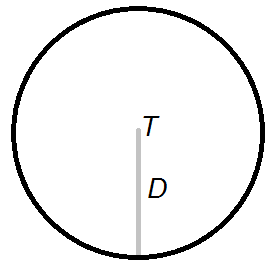
\includegraphics[height=0.25\textwidth]{img/Circle}
  \caption{An illustration of the circle with the radius given by the distance $D$ and the transmitter $T$ at its center.}
  \label{fig_circle}
\end{figure}

By measuring the distance from the receiver to another transmitter an additional circle can be calculated. Since the receiver must be situated on the perimeters of both circles it has to be located either at $A$ or $B$ as shown in Figure \ref{fig_2circles}.

\begin{figure}[H] 
  \centering
      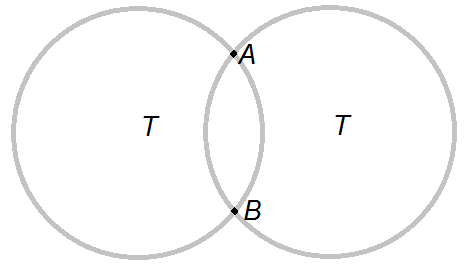
\includegraphics[height=0.25\textwidth]{img/2Circles}
  \caption{An illustration of two transmitters and their corresponding circles with intersections at $A$ and $B$ highlighted.}
  \label{fig_2circles}
\end{figure}

Repeating the previous step of measuring the distance to yet another transmitter it can be determined at which of the possible locations the receiver is situated since the three yielded circles all intersect in exactly one point as shown in Figure \ref{fig_3circles}.

\begin{figure}[H] 
  \centering
      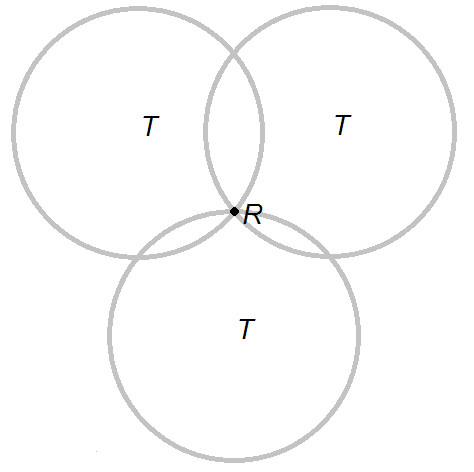
\includegraphics[height=0.45\textwidth]{img/3Circles}
  \caption{An illustration of three transmitters and the receiver shown in their intersection}
  \label{fig_3circles}
\end{figure}

\subsubsection{Application in 3-D}
Expanding the application the a 3-D environment increases the complexity as knowing only the distance between the receiver and one transmitter yields possible locations for the receiver on the peripheral of a sphere as shown in Figure \ref{fig_sphere}.
\begin{figure}[H] 
  \centering
      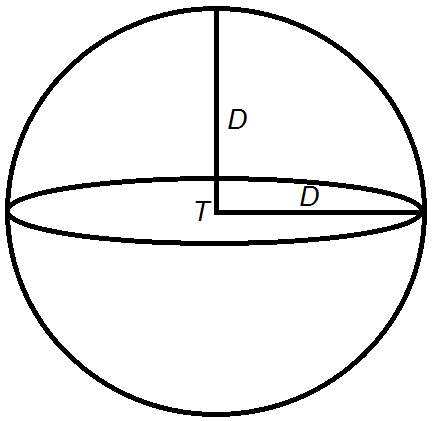
\includegraphics[height=0.25\textwidth]{img/Sphere}
  \caption{An illustration of the sphere with the radius given by the distance $D$ and the transmitter $T$ at its center.}
  \label{fig_sphere}
\end{figure}

By measuring the distance from the receiver to another transmitter an additional sphere can be calculated. Since the receiver must be situated on the peripheral of both spheres it has to be located somewhere on peripheral of the circle formed by the intersection of the two spheres as shown in Figure \ref{fig_2spheres}.

\begin{figure}[H] 
  \centering
      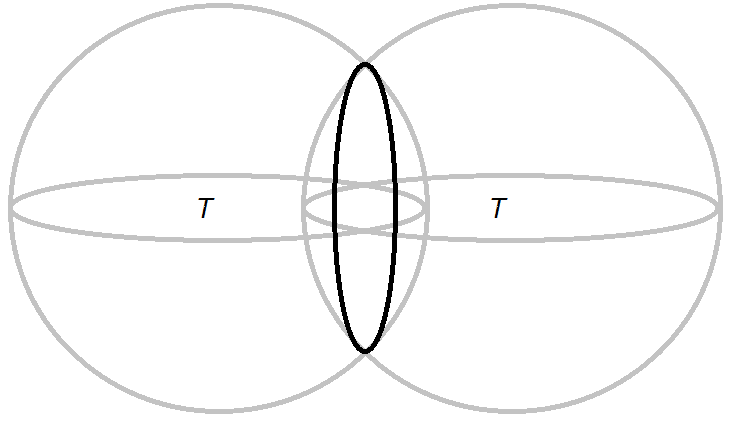
\includegraphics[height=0.25\textwidth]{img/2Spheres}
  \caption{An illustration of the two spheres and their intersection highlighted as a black circle.}
  \label{fig_2spheres}
\end{figure}

Having limited down the possible locations of the receiver to a circle, measuring the distance between the receiver and additional transmitters will decrease the possible locations in the same way as described in the 2-D environment at Section \ref{Trilateration2D}. That is, using a third transmitter limits the possible location of the receiver to two points and adding a fourth transmitter will pin the location of the receiver to single point.

%Explain ToA?

%Explain TWR?

\clearpage